%	Copyright (C) 2013 Systems Engineering Group
%
%	CHANGELOG:
%       2005-10-10 - corrected and extended. 
%       2013-01-28 - adjusted sections and explanation
%		2020-11-18 - basic content of hand-in


\documentclass[a4paper,10pt,twoside]{article}
\pagestyle{headings}
\usepackage{a4wide}
\usepackage{graphicx}
\graphicspath{ {./images/} }
\usepackage[colorlinks,hyperfigures,backref,bookmarks,draft=false]{hyperref}

\title{Disaggregated Compute and Storage for Distributed LSM-based Databases}
\author{Zidi Chen}
\date{\today}

\begin{document}

\maketitle

\begin{abstract}
Here you provide a very short intoduction into your topic and sum up your hand-in. 
It is important to highlight the main issues to be discussed in your hand-in here.
\end{abstract}

\tableofcontents

\section{Introduction of the Research Field}

Distributed databases like MongoDB, TiDB have been more widely used in many large-scale services senarios.
But in many cases, distributed databases could suffer performace degradation and low utilizationn from skew, backgroud operatio and compaction.
The paper~\textit{Hailstorm: Disaggregated Compute and Storage for Distributed LSM-based Databases} \cite{mainpaper}introduces Hailstorm, a system that disaggregates storage and compute for distributed LSM-based databases.
It shows that Hailstorm achieves load balance in many MongoDB deployments with skewed workloads, improving the average throughput by 60$\%$, while decreasing tail latency by as much as 5×.



\section{Basics}

\subsection{LSM-Tree}

Traditional disk-based index structures such as the B-tree will effectively double the I/O cost of the transaction to maintain an index such as this in real time, increasing the total system cost up to fifty percent. 
Hence Log-structured merge tree (LSM-Tree) has been widely used by many distributed databases, as it provides efficient indexing for a key-value store with a high rate of inserts and deletes.
The LSM-tree uses an algorithm that defers and batches index changes, cascading the changes from a memory-based component through one or more disk components in an efficient manner reminiscent of merge sort. 
During this process all index values are continuously accessible to retrievals (aside from very short locking periods), either through the memory component or one of the disk components.
It is a hybrid data structure, with a main memory layer (C0) placed on top of one or more filesystem layers (C1, and so on). 
In LSM-tree, updates are flushed down in batches, since this could reduce Disk I/O. 
Multiple updates on a given key may end up spread across C0 and any number of files in C1 (or below). 

\subsection{Skew in Distributed Databases}

Distributed databases \cite{mongodb,tidb} are designed for large-scale data storage, which usually run on multiple nodes in the same,
or even partitioned networks.
Distributed database use sharding to tore larger dataset and handle additional requests by distributing the data among multiple machines.
The database engine translates user queries into individual queries that are routed to one or multiple database instances for execution.
Therefore, the database may suffer skew issue, where keys are unevenly to different nodes, which could cause uneven access and some nodes may become the hotsopt.
This could lead to globally performance degradation.

\subsection{Compaction in LSM KV Stores}


As is shown in Figure. 1, if the insertion causes the C0 component to exceed a certain size threshold, a contiguous segment of entries is removed from C0 and merged into C1 on disk.  
\begin{figure}[h]
    \centering
	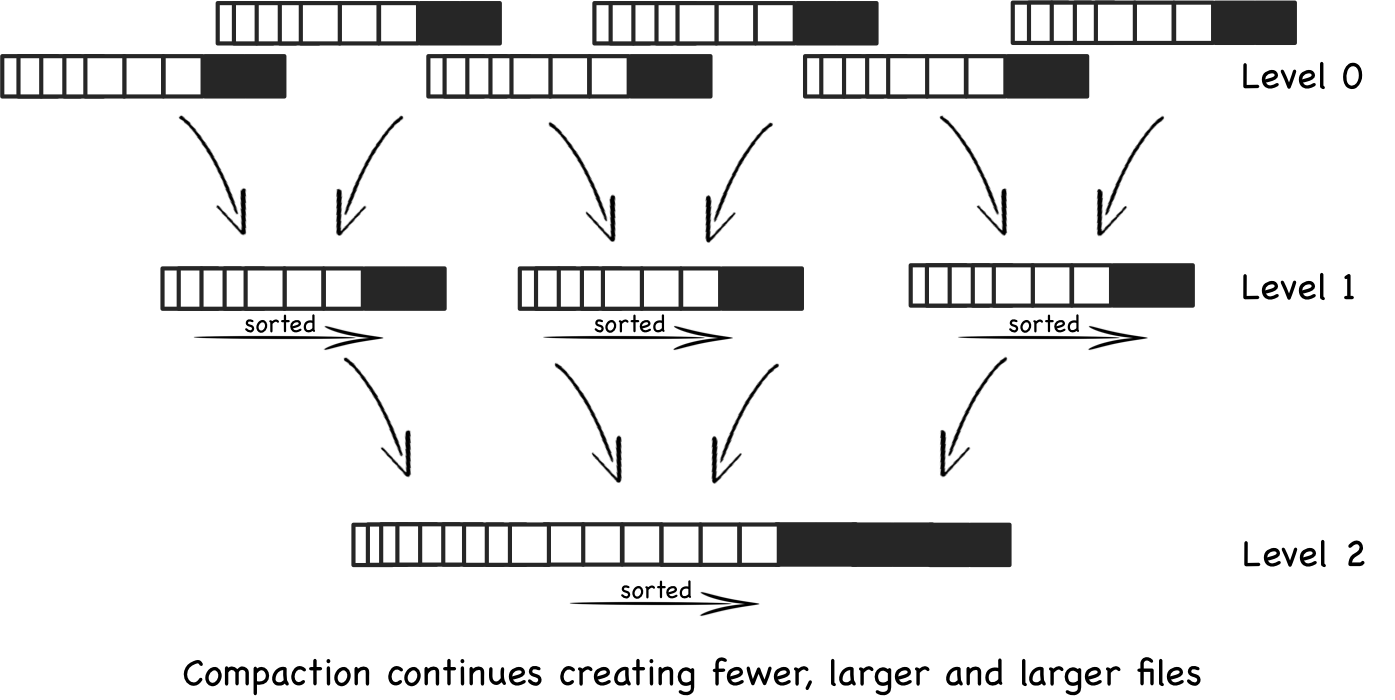
\includegraphics[scale=0.4]{LSM_Tree1.png}
    \caption{LSM Tree}
    \label{fig:mesh1}
\end{figure}



\section{Previous and Related Work}

Study the history of your topic by investigating its related work.
Compare the given paper to other publications dealing with the same research field.
Describe the shortcoming of existing approaches that will be solved or improved by the paper of your topic.

This is also the place to cite all sources and papers you have used in this handin and in your presentation. 
Bib\TeX$\!$ entries describing references are to be added to the \verb|refs.bib| file. 
You can find pre-formatted Bib\TeX$\!$ records in the Internet -- e.g. using the ACM Digital Library or Google Scholar.

\begin{quotation}
	``Sometimes you might want to use the \emph{quotation} environment in order to cite larger passages of the related work.''
\end{quotation}

\section{The Topic's Approach}

Describe the solution of the given paper, but do not copy it or repeat all of its details.
Present and explain the main concepts. 
%Do not forget to cite the paper~\cite{mainpaper} you have been assigned/chosen.
Note that you should rename this section. 

\section{Evaluation}

Present and discuss measurements, experiments, examples, ... but do not repeat the entire evaluation of the original paper.
\emph{Cite} all figures and tables copied form other papers.
You can keep this section short and focus on the aspects that were improved by the paper compared to existing approaches.

\section{Discussion}

What is bad about your paper? 
What are the good points? 
Mention criticism and ideas for improvement that you thought about while researching the topic.

\section{Conclusion}

Sum up your paper and the discussion points.

\bibliographystyle{unsrt}
\bibliography{handin} 

\end{document}
